\hsection{Loops}%
%
When we are working with sequences of data, we do not just want to perform an action on one data element.
We instead often want to apply the actions repetitively to all data elements.
Loops allow us to do just that, to perform the same actions multiple times.%
\pythonIdx{loop}%
%
\hsection{The \texttt{for} Loop Statement}%
%
\pythonIdx{loop!for}%
The most basic such sequence in \python\ may be the \pythonilIdx{for}~loop, which has the following pattern:%
%
\pythonSyntax{syntax/for_loop.py}%
%
\gitLoadAndExecPython{loops:for_loop_range}{}{loops}{for_loop_range.py}{}%
\listingPythonAndOutput{loops:for_loop_range}{%
An example of using the \pythonilIdx{for} loop over a \pythonilsIdx{range} of integer numbers.}{}%
%
\gitLoadAndExecPython{loops:for_loop_pi_liu_hui}{}{loops}{for_loop_pi_liu_hui.py}{}%
\listingPythonAndOutput{loops:for_loop_pi_liu_hui}{%
A variant of \cref{lst:variables:pi_liu_hui} which uses a \pythonilIdx{for} loop instead of five copies of the same instructions.}{}%
%
The keyword~\pythonilIdx{for} is followed by a loop variable.
Then comes the keyword~\pythonilIdx{in}, the \pythonil{sequence} we want to iterate over, and finally a colon~(\pythonilIdx{:}).
This variable will iteratively take on the values in the \pythonil{sequence}.
The loop body statements in the following, indented block are executed for each of these values.
Each time the body of the loop is executed is called an~\emph{iteration}\pythonIdx{iteration} of the loop.
After the loop, we leave one blank line followed by the code that will be executed after the loop completes.

In its most simple form, the \pythonilIdx{for} loop is applied to a \pythonilIdx{range} of integer numbers.
Ranges are sequences which work basically like slices\pythonIdx{slice} (see \cref{sec:lists,sec:strBasicOperations}).
\pythonil{range(5)} will give us a sequence of integers starting with~0 and reaching up to right \emph{before}~5, i.e., the integer range~\intRange{0}{4}.
\pythonil{range(6, 9)} gives the sequence of integers starting with~6 and stopping right \emph{before}~9, i.e., the integer range~\intRange{6}{8}.
Finally, \pythonil{range(20, 27, 2)} results in a sequence of integers that begins at~20, increments by~2 in each step, and ends right before~27.
This is the sequence~$(20, 22, 24, 26)$.
\pythonilsIdx{range}, like slices\pythonIdx{slice}, can also have negative increments:
The \pythonil{range(40, 30, -3)} starts with~40 and stops before reaching~30 and decrements by~3 in each step.
This is equivalent to the set~$(40, 37, 34, 31)$.

In \cref{lst:loops:for_loop_range}, we loop over exactly these ranges.
In this listing, we try to create a dictionary (see \cref{sec:dictionaries}) where some integer numbers are mapped to their squares.
We use four \pythonilIdx{for}~loops to fill this dictionary with data.
In each of these first four \pythonilIdx{for}~loops, we use \pythonil{i} as the loop variable.

When iterating over the \pythonil{range(5)} in the first loop, \pythonil{i} will hold the value \pythonil{0} in the first iteration (=~execution of the loop body).
The loop body \pythonil{squares[i] = i * i} will thus effectively be \pythonil{squares[0] = 0} and thus store the value~\pythonil{0} under key~\pythonil{0} into the dictionary \pythonil{squares}.
In the second iteration, \pythonil{i} will hold the value~\pythonil{1}.
Then, the body \pythonil{squares[i] = i * i} will effectively be \pythonil{squares[1] = 1}.
In the third iteration, \pythonil{i} will hold the value~\pythonil{2} and the body will perform \pythonil{squares[2] = 4}.
Next, \pythonil{i = 3} and \pythonil{squares[3] = 9} will be executed and in the laste iteration of the first loop, we store \pythonil{squares[4] = 16}.

In the second loop, which uses \pythonil{range(6, 9)}, \pythonil{i} will take on the values \pythonil{6}, \pythonil{7}, and \pythonil{8}, one by one.
The dictionary \pythonil{squares} will thus be extended with the values \pythonil{squares[6] = 36}, \pythonil{squares[7] = 49}, and \pythonil{squares[8] = 64}.
In the third loop, iterating over \pythonil{range(20, 27, 2)}, the following updates will be performed one by one \pythonil{squares[20] = 400}, \pythonil{squares[22] = 484}, \pythonil{squares[24] = 576}, and \pythonil{squares[26] = 676}.
In the fourth loop, \pythonil{i} takes on the values of the sequence \pythonil{range(40, 30, -3)}, which has the negative step length~\pythonil{-3}.
\pythonil{i} therefore first becomes~\pythonil{40}, then \pythonil{37} in the second iteration, then \pythonil{34}, and, finally,~\pythonil{31}.
We then print\pythonIdx{print} the dictionary and get the expected output in \cref{exec:loops:for_loop_range}.%
%
\bestPractice{underscore}{%
If we do not care about the value of a variable (or parameter), we should name it~\pythonil{_}\pythonIdx{\_}~\cite{PEP635}. %
This information is useful for other programmers as well as static code analysis tools.%
}%
%
At the end of \cref{lst:loops:for_loop_range} we show this special case:
We want to print\pythonIdx{print} \pythonil{"Hello World!"} three times.
Instead of copying the line \pythonil{print("Hello World!")} three times, we put it in a loop.
However, nowhere in the loop body we care about the value of the loop variable.
We thus simply call it \pythonil{_}\pythonIdx{\_}.
If we would not call it that, then another programmer seeing our code (or a static code analysis tool for that matter) could be confused as to why we do not use the loop variable.
Always remember that \inQuotes{real} code could be much more complicated, and any semantic hint we can include to convey our intentions will be helpful.

With these new tools at hand, we can revisit our program \cref{lst:variables:pi_liu_hui} for approximating~\numberPi\ from back in \cref{sec:approximatePiLiuHui}.
In this program, we executed the same code five times.
Instead of doing this, we can put this into a loop, which reduces the lines of code from over~25 to about~10 in \cref{lst:loops:for_loop_pi_liu_hui}.
The outputs in \cref{exec:variables:pi_liu_hui,exec:loops:for_loop_pi_liu_hui} are exactly the same.%
%
\FloatBarrier%
\endhsection%
%
\hsection{The \texttt{continue} and \texttt{break} Statements}%
%
\gitLoadAndExecPython{loops:for_loop_continue_break}{}{loops}{for_loop_continue_break.py}{}%
\listingPythonAndOutput{loops:for_loop_continue_break}{%
An example of the \pythonilIdx{continue} and \pythonilIdx{break} statements in a \pythonilIdx{for} loop.}{}%
%
Loops often have complex bodies, maybe containing conditional statements or other loops.
It is not an uncommon situation that, after performing some computations in the body of the loop, we already know that we can continue directly with the next iteration instead of executing the remainder of the loop body.
Sometimes we also find that we can entirely stop with the loop and continue with whatever instructions come after it, even if we did not yet exhaust the sequence over which we are iterating.
The former can be achieved using the \pythonilIdx{continue} and the latter with the \pythonilIdx{break} statement.

An example of both statements is given in \cref{lst:loops:for_loop_continue_break}.
Here, we iterate the variable~\pythonil{i} over the 15~values from~\pythonil{0} to~\pythonil{14}.
In the loop body, we first create a string~\pythonil{s} with the current value of~\pythonil{i} via the \pgls{fstring} \pythonil{f"i is now \{i\}."}
The very last instruction of the loop body, \pythonil{print(s)}\pythonIdx{print}, prints this string.

While \pythonil{i} would go from~\pythonil{0} to~\pythonil{14}, we actually want to abort the loop as soon as \pythonil{i} becomes greater than~\pythonil{10}.
Instead of modifying the \pythonilIdx{range} over which we loop (which would be reasonable), we here want to use the \pythonilIdx{break} statement.
We therefore wrap it into the conditional \pythonil{if i > 10:}, meaning that it will only be executed if~\pythonil{i > 10}.
As soon as \pythonilIdx{break} is reached, the loop will immediately be aborted.
No further instruction in the loop body is executed and no further iteration is performed.
Instead, the process will continue after the loop, with the line~\pythonil{print("All done.")}.

If \pythonil{i > 10} did not hold, the rest of the loop body is executed.
For the case that $\pythonil{i}\in\intRange{5}{8}$, we now want to directly jump to the next loop iteration by invoking the \pythonilIdx{continue}~statement.
This means that if \pythonil{i == 5}, the \pythonilIdx{continue}~statement lets the control directly return to the head of the loop, which will set~\pythonil{i = 6}.
This will happen until~\pythonil{i == 9}.
The condition \pythonil{5 <= i <= 8} is \emph{not} met for all $\pythonil{i}\in\intRange{0}{4}\cup\intRange{9}{15}$.
The next line, namely the \pythonil{print(s)}\pythonIdx{print}, can only be reached in these cases.
Of course, we already know that we will never even reach this code as soon as \pythonil{i == 11}.

As a result the program will print the string~\pythonil{s} only for~$\pythonil{i}\in\intRange{0}{4}\cup\{9, 10\}$ before finally outputting~\textil{All done.}.
This can be observed in the program output collected in \cref{exec:loops:for_loop_continue_break}.
With \pythonilIdx{break} and \pythonilIdx{continue}, we now have two tools that can help us to either abort any loop prematurely or to abort the current iteration of the loop prematurely (and continue with the next one, if any), respectively.%
%
\FloatBarrier%
\endhsection%
%
\hsection{Nesting Loops}%
%
\gitLoadAndExecPython{loops:for_loop_nested_primes}{}{loops}{for_loop_nested_primes.py}{}%
\listingPythonAndOutput{loops:for_loop_nested_primes}{%
Computing a list of all primes from \intRange{2}{200} using nested \pythonilIdx{for} loops.}{}%
%
Like conditional statements, \pythonilIdx{for}~loops can be arbitrarily nested.
Let us explore this by computing the list of all prime numbers less than~200 in \cref{lst:loops:for_loop_nested_primes}.%
%
\begin{definition}[Prime Number]%
A prime number~$p\in\naturalNumbersO$ is a positive integer~$p>1$ (greater than one) that has no positive integer divisors other than~$1$ and~$p$ itself~\cite{W2024MAWWR:PN,CP2005PNACP,R1994PNACMFF}.%
\end{definition}%
%
In our example program, we want to store all of these prime numbers in the list\pythonIdx{list} \pythonil{primes}.
We know that \pythonil{2} is a prime number and the only even one, so we directly initialize \pythonil{primes = [2]}, i.e., we set \pythonil{primes} to initially be a list only containing the integer~\pythonil{2}.
This will allow us to later on only consider the odd numbers in the range \intRange{3}{200}.
Just out of interest, we will count the total number of divisions that we need to perform until we have the full list of primes in the variable~\pythonil{n_divisions}.%
%
\begin{sloppypar}%
To find all primes in the integer set~\intRange{2}{200}, we let the loop variable \pythonil{candidate} iterate over~\pythonil{range(3, 200, 2)}\pythonIdx{range}.
This is the sequence of integer numbers starting~\pythonil{3} increasing with step length~\pythonil{2} and stopping right before~\pythonil{200}.
We know that even numbers (except~2) are not prime and we know that 200 is not a prime number either, so this should be OK.
Therefore, \pythonil{candidate} will iteratively become~\pythonil{3}, \pythonil{5}, \pythonil{7}, \dots, and eventually~\pythonil{195}, \pythonil{197}, and \pythonil{199}.
For each value of \pythonil{candidate}, we begin with the assumption that it is prime and then try to prove the opposite.
We set \pythonil{is_prime = True} then will try to find a divisor, in which case we will set \pythonil{is_prime = False}.
If we cannot find a divisor of \pythonil{candidate}, then \pythonil{is_prime} will remain \pythonil{True} and we can add \pythonil{candidate} to the list~\pythonil{primes}.
At least, this is the plan.%
\end{sloppypar}%
%
We will implement this idea with a nested inner loop.
Since the loop variable \pythonil{candidate} will always be odd, only odd numbers can be potential divisors.
Obviously, only integers greater than or equal to~\pythonil{3} are potential divisors.
We also only need to explore whether \pythonil{check} is a divisor of \pythonil{candidate} if it is not bigger than $\sqrt{\pythonil{candidate}}$.
If we had three integer numbers~$a$, $b$, and~$c$ such that $a=b*c$ and $b>\sqrt{a}$, then it must be that $c<\sqrt{a}$.
Since $a=\sqrt{a}*\sqrt{a}$ holds by definition, it would be impossible that $a=b*c$ if both $b>\sqrt{a}$ and $c\geq\sqrt{a}$.
Thus, if $b>\sqrt{a}$ was a divisor of $a$, then $c$ would also be a divisor of~$a$ that we would have found before reaching~$b$ in the loop since~$c<\sqrt{a}<b$.

Now, most integer numbers do not have integer square roots.
Since integer divisors cannot have fractions anyway, it is sufficient for us to use $\left\lfloor\sqrt{\pythonil{candidate}}\right\rfloor$.
In \python, such a \inQuotes{truncated} integer square root of an integer number~$\left\lfloor\sqrt{a}\right\rfloor$ can be computed using the \pythonilIdx{isqrt} function from the \pythonilIdx{math} module, which we \pythonilIdx{import} at the top of our program.

We can therefore iterate a second, inner loop variable \pythonil{check} over \pythonil{range(3, isqrt(candidate) + 1, 2)}\pythonIdx{range}\pythonIdx{isqrt}.
If \pythonil{candidate <= 3}, then this loop will never be executed because no number \pythonil{check} with $3\leq\pythonil{check}<\pythonil{candidate}$ exists.
Then, \pythonil{is_prime} will remain \pythonil{True} and we will add \pythonil{candidate} to \pythonil{primes} further down the outer loop body.
If \pythonil{candidate > 3}, then \pythonil{check} will go from $\pythonil{3}, \dots, \left\lfloor\sqrt{\pythonil{candidate}}\right\rfloor$.

In the body of our inner loop, we try to find out whether \pythonil{check} is an integer divisor of \pythonil{candidate}.
We can do this by computing the remainder of the division~$\pythonil{canddiate}/\pythonil{check}$.
Back in \cref{sec:int:integerArithmetics} we learned the \pgls{modulodiv} operator \expandafter\pythonilIdx{\%}, which does exactly that.
If \pythonil{candidate \% check} is~\pythonil{0}, then we can divide \pythonil{candidate} by \pythonil{check} without remainder.
Then, \pythonil{candidate} is divisible by \pythonil{check} and cannot be a prime number.
We thus can set \pythonil{is_prime = False}.
We can also immediately exit the inner loop using the \pythonilIdx{break} statement, because once we know that \pythonil{candidate} is not a prime number, we do not need to check further potential divisors.
(Notice that we also count all the \pgls{modulodiv} operations we perform by doing \pythonil{n_divisions += 1} at the beginning of the inner loop.)

After the inner loop, if \pythonil{is_prime} is still \pythonil{True}, we add \pythonil{candidate} to \pythonil{primes} by invoking the \pythonilIdx{append}\pythonIdx{list!append} method of the list.
Once we have completed the outer loop as well, we print the number~\pythonil{n_divisions} of divisions we have performed, the number~\pythonil{len(primes)}\pythonIdx{len}\pythonIdx{list!len} of prime numbers we have discovered and, finally, the list~\pythonil{primes} itself.
The output in \cref{exec:loops:for_loop_nested_primes} tells us that, after performing 252~divisions, we could identify 46~prime numbers inside~\intRange{2}{200}.%
%
\FloatBarrier%
\endhsection%
%
\hsection{Loops over Sequences}%
\label{sec:loopsOverSequences}%
%
\gitLoadAndExecPython{loops:for_loop_sequence}{}{loops}{for_loop_sequence.py}{}%
\listingPythonAndOutput{loops:for_loop_sequence}{%
An example iterating over the elements in different collection datastructures using \pythonilIdx{for} loops\pythonIdx{loop!for}.}{}%
%
When introducing the \pythonilIdx{for} loop\pythonIdx{for}\pythonIdx{loop!for}, we stated that it iterates over sequences of data.
We learned that \pythonilsIdx{range} are the most basic such sequences.
However, in \cref{sec:collections} we learned about collection datatypes, namely \pythonilsIdx{list}, \pythonilsIdx{tuple}, \pythonilsIdx{set}, and \pythonilsIdx{dict}.
The elements of all of these datatypes can be accessed sequentially, too.
This means that a \pythonilIdx{for} loop can iterate over them as well!

In \cref{lst:loops:for_loop_sequence} we illustrate how this is done:
It works exactly as if we were using \pythonilsIdx{range}.
In the program, we will build a list~\pythonil{txt} with strings that we will later write to the output.

First, we want to iterate over a list\pythonIdx{list}~\pythonil{lst} containing the four integers~\pythonil{[1, 2, 3, 50]}.\pythonIdx{list!iterate over}
This is done by simply writing \pythonil{for i in lst}.
Here, \pythonil{i} is the loop variable and it will step-by-step take on all the values in~\pythonil{lst}, one by one.
In the body of this loop, we invoke \pythonil{txt.append(f"i=\{i\}")}.
The \pgls{fstring} will evaluate to \pythonil{"i=1"} in the first iteration, to \pythonil{"i=2"} in the second, to \pythonil{"i=3"} in the third, and to \pythonil{"i=50"} in the fourth and last iteration of this loop.
These strings are appended to the list \pythonil{txt} via the \pythonilIdx{append}\pythonIdx{list!append} method.

Then we move on and want to iterate over a tuple\pythonIdx{tuple}~\pythonil{tp}, which contains three floating point numbers, namely~\pythonil{(7.6, 9.4, 8.1)}.\pythonIdx{tuple!iterate over}
This works exactly in the same way:
\pythonil{for f in tp} will let the loop variable~\pythonil{f} take on the values \pythonil{7.6}, \pythonil{9.4}, and finally~\pythonil{8.1}.
We again append\pythonIdx{list!append}\pythonIdx{append} their textual representation to the list \pythonil{txt}, this time using the \pgls{fstring} \pythonil{f"f=\{f\}"}.

As third example, we create the set\pythonIdx{set}~\pythonil{st} containing the three strings~\pythonil{\{"u", "v", "w"\}}.\pythonIdx{set!iterate over}
We can do this again by simply writing \pythonil{for s in st}, which lets the loop variable~\pythonil{s} take on the values \pythonil{"w"}, \pythonil{"u"}, and \pythonil{"v"}, \emph{in an arbitrary order}.
Remember that sets in \python\ are unordered (see \cref{bp:setsUnordered}), which means that if we run the program twice, we may get different results.
Either way, we can iterate over all the values in the set~\pythonil{st}.
We again want to store these values as nicely formatted strings in~\pythonil{txt}.
This time we use the \pgls{fstring} \pythonil{f"s=\{s!r\}"}\pythonIdx{"!r}.
Notice the \pythonil{!r} format specifier\pythonIdx{"!r}:
It will print the \emph{representation} of the string~\pythonil{s}, which basically means to put quotation marks (and to potentially escape\pythonIdx{str!escaping}\pythonIdx{escaping} otherwise unprintable characters, see \cref{sec:str:escaping}).
Thus, we will add \pythonil{"s='v'"}, \pythonil{"s='u'"}, and~\pythonil{"s='w'"} to \pythonil{txt} (in an arbitrary order).

As fourth and final example, we create a dictionary~\pythonil{dc}\pythonIdx{dict} that maps floating point numbers to Boolean values, containing the two entries, namely~\pythonil{\{1.1: True, 2.5: False\}}.\pythonIdx{dict!iterate over}
Now a dictionary is a bit special:
It maps keys to values.
When working with the whole dictionary datastructure~\pythonil{dc} as a collection, then we can access it in three ways:
%
\begin{enumerate}%
%
\item Iterating over \pythonil{dc} directly lets us view all the keys in the dictionary~\pythonil{dc}. %
This is equivalent to iterating over \pythonil{dc.keys()}\pythonIdx{dict!keys}.%
%
\item Iterating over \pythonil{dc.values()}\pythonIdx{dict!values} lets us access all the values in the dictionary~\pythonil{dc}.%
%
\item Iterating over \pythonil{dc.items()}\pythonIdx{dict!items} lets us access all key-value pairs in the dictionary~\pythonil{dc} as tuples.%
\end{enumerate}%
%
In our example program, we apply all of these methods.
We iterate over the keys in~\pythonil{dc} via \pythonil{for k in dc}, which lets \pythonil{k} take on the values \pythonil{1.1} and \pythonil{2.5}, one after the other.
We iterate over the values in~\pythonil{dc} via \pythonil{for v in dc.values()}, which lets \pythonil{v} take on the values \pythonil{True} and \pythonil{False}, one after the other.%
%
\begin{sloppypar}%
Finally, we iterate over all key-value pairs.
Look closely at this one:
We \emph{could} write \pythonil{for t in dc.items()}, which would let a loop variable~\pythonil{t} take on the tuple values \pythonil{(1.1, True)} and then \pythonil{2.5: False}.
However, back in \cref{sec:tuples}, we learned about tuple unpacking\pythonIdx{tuple!unpacking}\pythonIdx{unpacking}.
So instead, we write \pythonil{for k, v in dc.items()}.
This is a shortcut for writing \pythonil{for t in dc.items()} followed by \pythonil{k, v = t}.
It directly unpacks the tuples in the sequence \pythonil{dc.items}, meaning that we get pairs of \pythonil{k=1.1}, \pythonil{v=True} and \pythonil{k=2.5}, \pythonil{v=False}.
All of them are again appended to our text list~\pythonil{txt}.%
\end{sloppypar}%
%
After all of these loops, we have ended up with a list~\pythonil{txt} containing~16 strings.
We want to combine all of them to a single string, using \pythonil{", "} as a separator.
We could do this in another loop.
However, \python\ offers us a much more efficient shorthand for this:
The method \pythonilIdx{join}\pythonIdx{str!join} of the class~\pythonilIdx{str}.

For any string~\pythonil{z}, \pythonil{z.join(seq)} accepts a sequence \pythonil{v} of strings.
It then concatenates all the strings in \pythonil{seq}, placing \pythonil{z} as separator between any two strings.
Thus, invoking \pythonil{", ".join(txt)} produces \textil{i=1, i=2, i=3, i=50, f=7.6, f=9.4, ...}.
This text is finally is written to the output via the \pythonilIdx{print} function, giving us the results shown in  \cref{exec:loops:for_loop_sequence}.

\gitLoadAndExecPython{loops:for_loop_sequence_primes}{}{loops}{for_loop_sequence_primes.py}{}%
\listingPythonAndOutput{loops:for_loop_sequence_primes}{%
Computing a list of all primes from \intRange{2}{200} using nested \pythonilIdx{for} loops. %
Compared to \cref{lst:loops:for_loop_nested_primes}, this program is more efficient because it only tests primes as divisors.%
}{}

Let us now use this new ability to iterate over collection datastructures to improve upon our prime number enumeration program \cref{lst:loops:for_loop_nested_primes}.
Back when writing that program, we immediately stored \pythonil{2} as a prime into our list~\pythonil{primes}.
We then only tried the odd numbers less than~200 as potential prime number \pythonils{candidate}.
For each potential prime number \pythonil{candidate}, we tested all (odd) numbers~\pythonil{check} from the range \pythonil{range(3, isqrt(candidate) + 1, 2)}\pythonIdx{range} as possible divisors.

When thinking about this, we realize that actually, only the prime numbers in this range are interesting.
For example, we do never need to check whether \pythonil{candidate} is divisible by~9, because we will have already checked whether it can be divided by~3.
We also never need to check whether we can divide it by~55, because we will have already checked~5.

Therefore, in our new and more efficient program \cref{lst:loops:for_loop_sequence_primes}, we replace the head of the inner loop with~\pythonil{for check in primes[1:]:}.
\pythonil{primes[1:]} is a slice\pythonIdx{list!slicing}\pythonIdx{slicing}\pythonIdx{slice} of the list~\pythonil{primes} containing all but the first element (see \cref{sec:lists}).
This first element is~\pythonil{2}, and since all \pythonils{candidate} are odd, we do not need to try whether they can be divided by~\pythonil{2}.
The outer loop will step-by-step add prime numbers to \pythonil{primes}.
Actually, for each value of the loop variable \pythonil{candidate}, \pythonil{primes} will contain all prime numbers which are smaller than \pythonil{candidate}.
We only need to check those which are less than or equal to \pythonil{isqrt(candidate)}\pythonIdx{isqrt}, so we store this value in a new variable \pythonil{limit} to avoid re-computing it in the inner loop.
The \pythonilIdx{break} statement lets us exit the inner loop as soon as we hit this limit.

The lists of primes that our programs generate in \cref{exec:loops:for_loop_sequence_primes,exec:loops:for_loop_nested_primes} are exactly the same.
However, our new program needs to perform only 224~divisions instead of~252.

Later, in \cref{sec:iteration}, we will learn that loops in \python\ can be applied to the more general concept of~\pythonilsIdx{Iterator}.
We will also see how the \pythonilIdx{for}~keyword can be used to construct sequences via a process called \emph{comprehensions}.%
%
\FloatBarrier%
\endhsection%
%
\hsection{Enumerating over Sequences when needed Indices}%
\label{sec:enumOverSequences}%
%
\gitLoadAndExecPython{loops:for_loop_no_enumerate}{}{loops}{for_loop_no_enumerate.py}{}%
\listingPythonAndOutput{loops:for_loop_no_enumerate}{%
Enumerating over the index-value pairs of a list (inefficiently).}{}%
%
Assume that we have a list \pythonil{data} of integer values~\pythonil{v}.
If we want to iterate over all the values~\pythonil{v} in~\pythonil{data}, then \pythonil{for v in data} would do the trick.
However, what if we also want to know the current index~\pythonil{i} for each data element during the iteration?
Then this construct no longer works.

We basically have two choices:
As first option, we can iterate over \pythonil{data} by accessing the elements by their index~\pythonil{i} directly.
In this case, we would use a \pythonilIdx{range} that goes from~\pythonil{0} to \pythonil{len(data) - 1}\pythonIdx{len}\pythonIdx{list!len}.
The head of the loop now looks like this:~\pythonil{for i in range(len(data))}.
The data values~\pythonil{v} are then accessed via~\pythonil{data[i]}.
This is illustrated in \cref{lst:loops:for_loop_no_enumerate}.

The drawback of this method is that it will \emph{only} work for \pythonilsIdx{list}, because among the collection datastructures discussed so far, only \pythonilsIdx{list} are directly indexable.
Therefore, the second option to achieve our goal would be to use an additional integer variable~\pythonil{i} which we would initialize as \pythonil{i: int = 0} before the loop.
 We would then increment it as~\pythonil{i += 1} at the bottom of the loop body, where \pythonil{i += 1} is equivalent to \pythonil{i = i + 1}\pythonIdx{+=}\pythonIdx{+}.
This would work with all collection classes.

Both options are a bit iffy, as they introduce more and less readable additional code.
There is a third option, though.
And because I advocate using static code analysis tools, I let another such tool discover this option for us.%
%
\begin{figure}%
\centering%
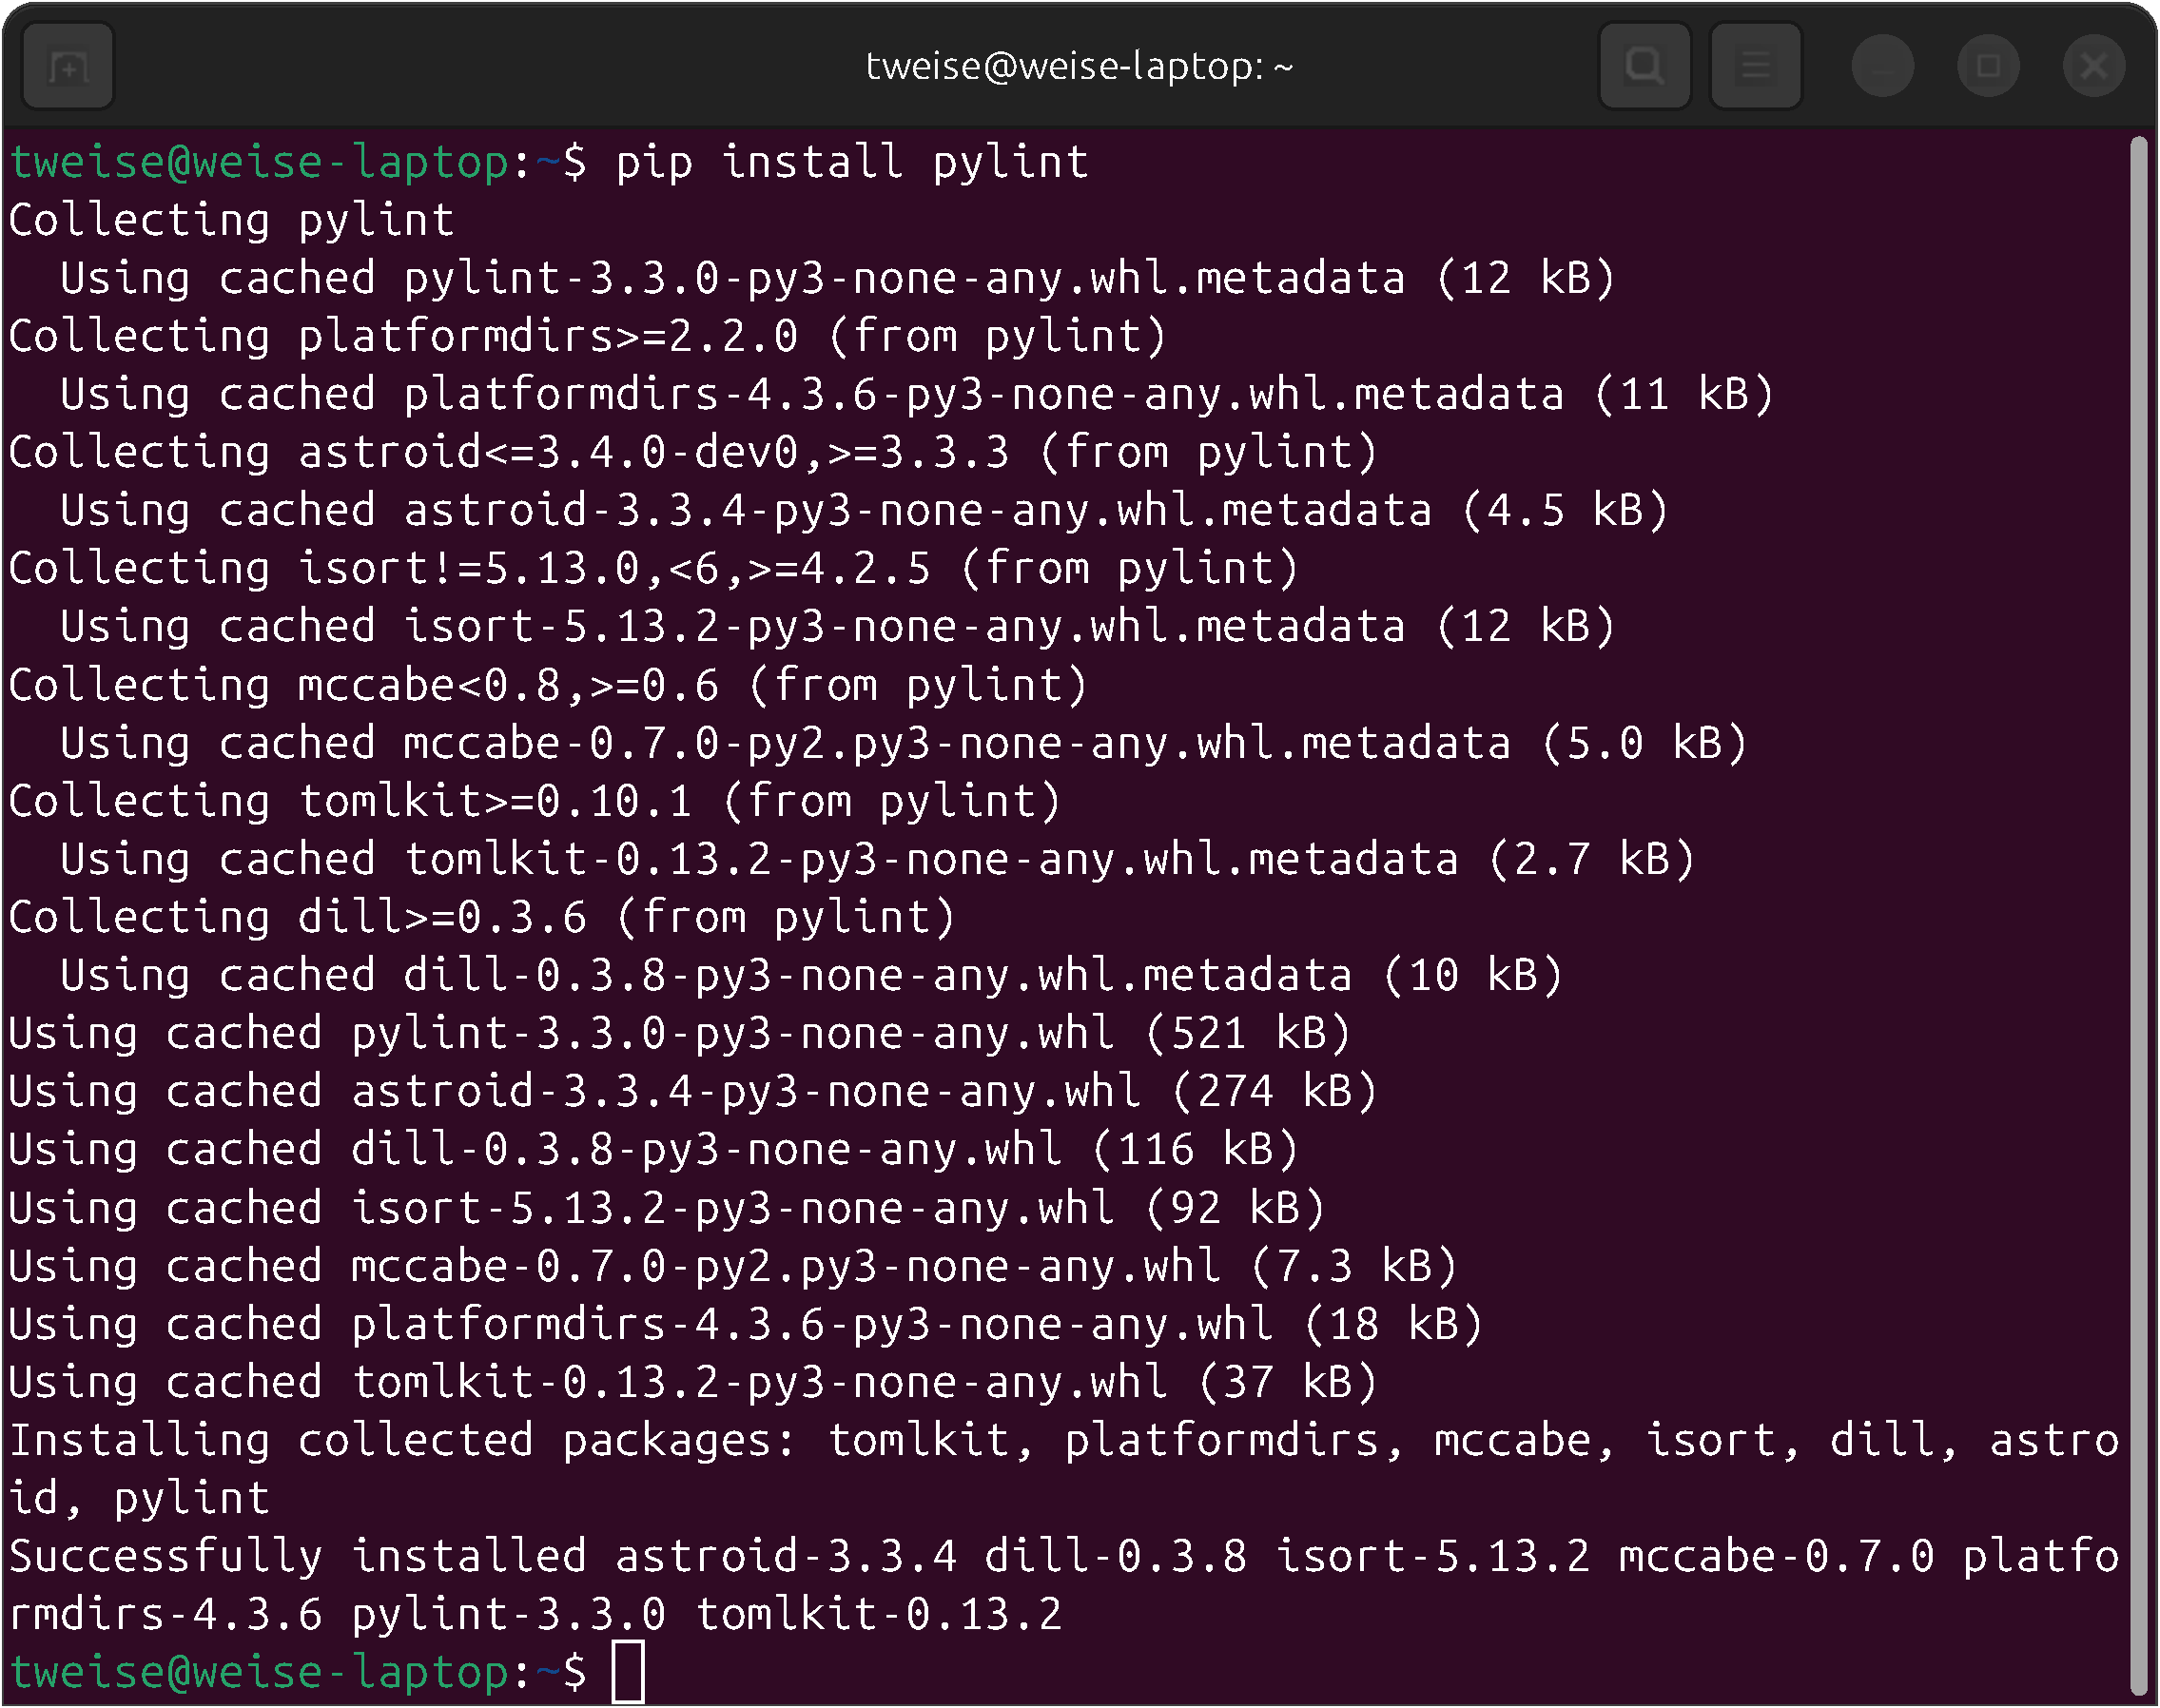
\includegraphics[width=0.7\linewidth]{\currentDir/pipInstallPylint}%
\caption{Installing \pylint\ in a \ubuntu\ \pgls{terminal} via \pip~(see \cref{sec:pipAndVenv} for a discussion of how packages can be installed).}%
\label{fig:pipInstallPylint}%
\end{figure}%
%
\usefulTool{pylint}{%
\pylint\ is a \python\ \pgls{linter} that analyzes code for style, potential errors, and possible improvements~\cite{PC2024PL}. %
It can be installed via \bashil{pip install pylint} as shown in \cref{fig:pipInstallPylint} on \cpageref{fig:pipInstallPylint}. %
You can then apply \pylint\ using the command \bashil{pylint fileToScan.py}. %
We provide a script for using \pylint\ with a reasonable default configuration in \cref{lst:bash:pylint} on \cpageref{lst:bash:pylint}.%
}%
%
\gitExec{exec:loops:for_loop_no_enumerate:pylint}{\programmingWithPythonCodeRepo}{.}{_scripts_/pylint.sh loops for_loop_no_enumerate.py}%
\listingToolOutput{loops:for_loop_no_enumerate:pylint}{%
The results of static code analysis using the \pylint\ \pgls{linter} for the program given in \cref{lst:loops:for_loop_no_enumerate}.}%
%
\gitLoadAndExecPython{loops:for_loop_enumerate}{}{loops}{for_loop_enumerate.py}{}%
\listingPythonAndOutput{loops:for_loop_enumerate}{%
Enumerating over the index-value pairs of a list using the \pythonilIdx{enumerate} function.}{}%
%
In \cref{exec:loops:for_loop_no_enumerate:pylint}, \pylint\ suggest that we should iterate over the list \pythonil{data} using the \pythonilIdx{enumerate} function.
\pythonilIdx{enumerate} accepts a collection as parameter and creates a sequence of index-value tuples.
Since we can unpack such tuples while iterating over this sequence (see \cref{lst:loops:for_loop_sequence})\pythonIdx{tuple!unpacking}\pythonIdx{unpacking}, the head of our loop now takes on the form \pythonil{for i, v in enumerate(data)}.
Notice that the index~\pythonil{i} comes first and the value~\pythonil{v} comes second in this unpacked-tuple-based enumeration.
This is implemented in \cref{lst:loops:for_loop_enumerate}.
And it would work exactly the same, regardless whether \pythonil{data} was a list, set, tuple, or dictionary.

Now, above we used the \pylint\ \pgls{linter} to discover that we could improve our code by using this concept.
At the time of this writing, \ruff\ and \mypy\ did not find this potential improvement.
Maybe their future versions will.
Regardless, it becomes clear that using more static analysis tools is always a good idea, as stated back in \cref{bp:manyCodeAnalysisTools}.%
%
\FloatBarrier%
\endhsection%
%
\hsection{The \texttt{while} Loop}%
\label{sec:whileLoop}%
%
Old clay tablets show that the Babylonians were able to approximate~$\sqrt{2}$ maybe as far back as 4000~years ago~\cite{FR1998SRAIOBMY7IC,S2011NA:NA}.
The mathematician Hero(n) of Alexandria, who lived in the first century~\pgls{CE}, specified an abstract algorithm for computing the square root of numbers which, today, is known as Heron's Method~\cite{S2011NA:NA,K2009BMOCTSRJBOFTAOCC}.

Given a number~$a$ and aiming to find the square root~$\sqrt{a}$ of~$a$, this algorithm starts with a guess~$x_0$, let's say~$x_0=1$.
In each iteration~$i$, it will compute a new guess as follows~\cite{S2011NA:NA,K2009BMOCTSRJBOFTAOCC}:%
%
\begin{equation}%
x_{i+1}=\frac{1}{2}\left(x_i+\frac{a}{x_i}\right)%
\label{eq:heronGuessUpdate}%
\end{equation}%
%
We can roughly imagine that the algorithm works as follows:
If $x_i$ was too big, i.e., $x_i>\sqrt{a}$, then~$\frac{a}{x_i}<\sqrt{a}<x_i$.
If $x_i$ was too small, i.e., $x_i<\sqrt{a}$, then $\frac{a}{x_i}>\sqrt{a}>x_i$.
By computing the average of~$x_i$ and~$\frac{a}{x_i}$ as the next guess, we hope to approach~$\sqrt{a}$.
If $x_i=\sqrt{a}$, then $\frac{a}{x_i}=\sqrt{a}$ by definition and~$x_{i+1}=x_i$.
Showing that this actually works and that the error gets smaller over time is more complicated~\cite{S2011NA:NA}.

If we want to implement this algorithm, we will naturally need a loop of some sort.
Clearly, we perform the same computation again and again.
However, a \pythonil{for}~loop will not do:
We do not know the number of steps that we will need in advance.
Of course, we could try to pick a very very huge number and then \pythonil{break} the loop when the guesses converg {\dots} but that is just ugly.
The \pythonilIdx{while} comes to rescue:%
%
\pythonSyntax{syntax/while_loop.py}%
\FloatBarrier%
%
\gitLoadAndExecPython{loops:while_loop_sqrt}{}{loops}{while_loop_sqrt.py}{}%
\listingPythonAndOutput{loops:while_loop_sqrt}{%
We compute the square root of a number using Heron's Method~\cite{S2011NA:NA,K2009BMOCTSRJBOFTAOCC} implemented as py \pythonilIdx{while} loop.}{}%
%
In the \pythonilIdx{while} loop, the body is executed as long as a Boolean expression in the head of the loop evaluates to~\pythonilIdx{True}.
We now use this new construct to implement Heron's Method in \cref{lst:loops:while_loop_sqrt} and use it to compute the square roots of~0.5, 2, and~3.

We begin the program with an outer \pythonil{for} loop that iterates a variable~\pythonil{number} over the \pythonil{float} values \pythonil{0.5}, \pythonil{2.0}, and~\pythonil{3.0}.
We want to apply the algorithm to each of these values.
We use two variables~\pythonil{guess} be the current guess of what $\sqrt{\pythonil{number}}$ could be and \pythonil{old_guess} be the previous guess.

We initialize \pythonil{guess} with \pythonil{1.0} and \pythonil{old_guess} with a different value, say~\pythonil{0.0}.
Our \pythonilIdx{while} loop should keep iterating as long as~\pythonil{guess != old_guess}.
Of course, if we could represent real numbers at infinite precision, we would never reach \pythonil{guess == old_guess} for any \pythonil{number} with an irrational square root.
However, the \pythonil{float} datatype has limited precision (see \cref{sec:howFloatingPointNumbersWork}).
Therefore, at least in our examples, \pythonil{guess != old_guess} indeed eventually becomes~\pythonilIdx{False}.%
%
\bestPractice{noFloatEqualAsCondition}{%
Do not use (un)equality comparisons of \pythonils{float} as loop termination criteria, as they may lead to endless loops. %
There can always be inputs that cause endless oscillations between values or the appearance of \pythonilIdx{nan} values (see \cref{sec:float:special}).%
}%
%
The only reason why we did it here is that it looks nice and is easy to read as a functional and yet brief example of a \pythonilIdx{while} loop.\footnote{%
To enforce that no oscillation between two neighboring \pythonil{float} values could occur, one could use the condition \pythonil{abs(old_guess - guess) / max(old_guess, guess) >= 1e-15} instead. %
This makes the loop stop when the relative difference between \pythonil{guess} and \pythonil{old_guess} becomes less than~$10^-{15}$.%
}%
Anyway, the loop condition necessitates us to store some value different from~\pythonil{1.0} in \pythonil{old_guess} initially (and we picked~\pythonil{0.0}).
In the loop, first the current guess becomes the old guess via \pythonil{old_guess = guess}.
Then we update the guess as specified in \cref{eq:heronGuessUpdate}, by setting \pythonil{guess = 0.5 * (guess + number / guess)}.

Finally, we print the result of the computation, and for the sake of comparison, we also print the output of the \pythonilIdx{sqrt} function of the \pythonilIdx{math} module.
As you can see, our algorithm delivers almost the same result.
It works quite well, at very high precision.
Also, notice how we used the Unicode escape method from \cref{sec:unicodeChars} to represent the characters~$\sqrt{\cdot}$ and~$\approx$ as \textil{\\u221A} and \textil{\\u2248} to get them printed on the console.%
%
\FloatBarrier%
\endhsection%
%
%
\hsection{The \texttt{else} Statement at the Bottom of Loops}%
\label{sec:loopElse}%
%
Now, you have learned before that we can leave a loop body immediately by calling the~\pythonilIdx{break} statement.
Let's say that we want to perform a certain action \emph{after} the loop if the loop has completed normally, i.e., if \pythonilIdx{break} was not invoked.
We can do this by declaring a Boolean variable denoting whether the loop has completed normally before the loop and initializing it with \pythonil{True}.
If we invoke \pythonilIdx{break}, then we would first set this variable to \pythonil{False}.
After the loop, we could place an \pythonil{if} to check if the variable is still \pythonil{True} and then execute the action.
This is totally fine, but \python\ offers us a much less verbose method:
Using the \pythonilIdx{else} statement at the bottom of the loop, which works for both \pythonilIdx{for} and \pythonilIdx{while} loops:%
%
\pythonSyntax{syntax/for_loop_else.py}%
\pythonSyntax{syntax/while_loop_else.py}%
%
\gitLoadAndExecPython{loops:while_loop_search}{}{loops}{while_loop_search.py}{}%
\listingPythonAndOutput{loops:while_loop_search}{%
We implement binary search~\cite{K1998SAS,H2024POIC:BS,B1999PP} using a \pythonilIdx{while} loop with a \pythonilIdx{break} statement.}{}%
%
We now use this construct to implement a binary search~\cite{K1998SAS,H2024POIC:BS,B1999PP}.
Binary search works is an algorithm that finds the index of an element in a \emph{sorted} sequence \pythonil{data} of values.
The core concept of binary search is that we consider a segment~$S$ of the list in which the element~$E$ we search may be contained.
In each step of the algorithm, we want to reduce the size of this segment by ruling out the \emph{half} in which~$E$ cannot be.
We do this looking at the element~$M$ right in the middle.
Now, the whole sequence~\pythonil{data} and, hence, also the segment~$S$, are sorted.
If~$M$ is bigger than~$E$, then $E$ must be in the lower half, i.e., in the sub-segment from the start of~$S$ to right before~$M$.
If~$M$ is smaller than~$E$, then $E$ must be in the upper half, i.e., in the sub-segment starting right after~$M$ and reaching until the end of~$S$.
Otherwise, we must have found the element.
This means in one step we have effectively halved the size of~$S$.
If~$n=\pythonil{len(data)}$, then we can do this at most $\log_2 n$~times and the time complexity of binary search is in~\bigOb{\log n}~\cite{K1998SAS,H2024POIC:BS,B1999PP}.%
%
\begin{sloppypar}%
In~\cref{lst:loops:while_loop_search}, we want to find the indices of some characters in the alphabetically sorted string~\pythonil{data = "abdfjlmoqsuvwyz"}.
Of course, there is the \pythonilIdx{find}\pythonIdx{str!find} method that can do this, but we want to take advantage of the fact that the characters in \pythonil{data} are sorted.
We search for the six characters~\pythonil{"a"}, \pythonil{"c"}, \pythonil{"o"}, \pythonil{"p"}, \pythonil{"w"}, and~\pythonil{"z"}.
Four of them are in \pythonil{data}, but \pythonil{"c"} and \pythonil{"p"} are not.
To search them anyway, we let a variable \pythonil{search} iterate over the list \pythonil{["a", "c", "o", "p", "w", "z"]}.%
\end{sloppypar}%
%
Now in the inner loop, we implement the binary search.
This search will maintain and update two indices \pythonil{lower} and \pythonil{upper}.
\pythonil{lower} is the inclusive lower end of the segment in which \pythonil{search} could be contained.
It is therefore initialized with~\pythonil{0}.
\pythonil{upper} is the exclusive upper end of the segment in which \pythonil{search} could be contained.
We initialize it with \pythonil{len(data)}; as it is \emph{exclusive}, it will be 1 bigger than the largest valid index \pythonil{len(data) - 1}.
Our segment is not empty, i.e., contains at least one element, as long as \pythonil{lower < upper}.
This is therefore the loop condition of the inner loop.

Inside the binary search loop, we first compute the mid index as \pythonil{mid = (lower + upper) // 2}\footnote{%
Interestingly, this works only because \python~3 has integers of infinite range (see \cref{sec:int}). %
In programming languages like \pgls{C} or \pgls{Java} where integer types have limited ranges, we need to do \pythonil{mid = lower + (upper - lower) // 2}~\cite{H2024POIC:BS}.%
}.
We obtain the value \pythonil{mid_str} as the single character at that index via \pythonil{mid_str = data[mid]}.

We know that if \pythonil{mid_str < search}, then our character \pythonil{search} cannot be located at any index in the range~\intRange{0}{\pythonil{mid}}.
So in this case, we can update the \emph{inclusive} index \pythonil{lower} to become \pythonil{mid + 1}.
Otherwise, if \pythonil{mid_str > search}, then we know that \pythonil{search} could not possibly located anywhere in the range~\intRange{\pythonil{mid}}{\pythonil{len(data) - 1}}.
We thus would set the \emph{exclusive} index \pythonil{upper} to \pythonil{mid}, which excludes all items starting at index \pythonil{mid} from further consideration.%
%
\begin{sloppypar}%
Now if neither \pythonil{mid_str < search} nor \pythonil{mid_str > search} were \pythonil{True}, it must be that \pythonil{mid_str == search}.
This means that we found the location of \pythonil{search} -- it is at the index~\pythonil{mid}.
Therefore, we print this result to the output.
(Notice that the \pythonil{!r}\pythonIdx{"!r} format specifiers in the \pgls{fstring} we use add the nice single quotes around \pythonil{search} and \pythonil{data}.)
After printing the information, we exit the \pythonilIdx{while} loop using the \pythonilIdx{break} statement.%
\end{sloppypar}%
%
Now, there is the possibility that we cannot find \pythonil{search} in \pythonil{data} because it is simple in there.
In this case, we will never print the output and also not leave the loop with \pythonilIdx{break}.
In each iteration that does not end with \pythonilIdx{break}, we will either increase \pythonil{lower} or decrease \pythonil{upper}.
Thus, eventually \pythonil{lower < upper} will become \pythonil{False}.
This is when the \pythonilIdx{else} statement at the bottom of the loop is executed.
Then and only then we print that we did not find the string.%
\endhsection%
%
\hsection{Summary}%
With this, we depart from the subject of loops.
We have learned two ways to execute code iteratively:
The \pythonilIdx{for} loop iterates of sequences of objects, which can either be \pythonilsIdx{range} of numbers or arbitrary collections.
The \pythonilIdx{while} loop permits us to specify an arbitrary Boolean expression as loop condition.
In the bodies of both loops, we can jump to the next iteration at any time using the \pythonilIdx{continue} statement or we can exit the loops entirely using the \pythonil{break} statement.
Finally, placing an \pythonilIdx{else} statement at the bottom of the loop allows us to execute some code when the loop completes regularly, i.e., not via~\pythonilIdx{break}.

We now have some nice tools in our hands.
We can create code that branches and conditionally performs actions via \pythonil{if}-\pythonil{else}.
And we can repeatedly perform actions via \pythonil{for} and \pythonil{while}.
Our examples also have become more elaborate and interesting.
We can now approximate~\numberPi\ with arbitrarily many steps of the approach of LIU Hui~(刘徽).
We can implement Heron's Method to compute the square root of a number and we perform binary search over arbitarily large (sorted) data.
We can do quite a lot!

What we cannot yet do is to have a block of code that we want to re-use in \emph{different} places.%
\endhsection%
%
\FloatBarrier%
\endhsection%
%
